\documentclass[aspectratio=1610]{beamer}
\hypersetup{
        unicode=true,
        linkcolor=blue,
        anchorcolor=blue,
        citecolor=green,
        filecolor=black,
        urlcolor=blue
    }

%%%%% PACKAGES HERE
%% \usepackage{}
\usepackage{amsmath}
\usepackage{amssymb}
\usepackage{listings}
\usepackage[cache=false]{minted}
\usepackage{textcomp}
\usepackage{subcaption}


\usepackage[style=authortitle,backend=biber]{biblatex}
\addbibresource{references.bib}

%%%%%%%%%%%%%%%%%%%%%%%%%%%%%%%%%%%
%% DO NOT CHANGE

\usetheme{default}
\useinnertheme{circles}
\useoutertheme{infolines}
\usefonttheme{serif}

\usepackage{etoolbox}

%% T for navigation symbols
%%\setbeamertemplate{navigation symbols}{}

%% T for header
%% \setbeamertemplate{headline}{%
%%   \leavevmode%
%%   \ifdefempty{\insertsubsectionhead}{
%%     \begin{beamercolorbox}[wd=0.99\paperwidth,ht=2.25ex,dp=1ex,center]{section in head/foot}%
%%       % \hbox to .5\paperwidth{\hfil\insertsectionhead\hfil}
%%       \insertsectionhead
%%     \end{beamercolorbox}%
%%   }{
%%     \begin{beamercolorbox}[wd=.44\paperwidth,ht=2.25ex,dp=1ex,right]{section in head/foot}%
%%       % \hbox to .5\paperwidth{\hfil\insertsectionhead\hfil}
%%       \insertsectionhead
%%     \end{beamercolorbox}%
%%     \begin{beamercolorbox}[wd=.1\paperwidth,ht=2.25ex,dp=1ex,center]{section in head/foot}%
%%       % \hbox to .5\paperwidth{\hfil\insertsectionhead\hfil}
%%       -
%%     \end{beamercolorbox}%
%%     \begin{beamercolorbox}[wd=.44\paperwidth,ht=2.25ex,dp=1ex,left]{subsection in head/foot}%
%%       % \hbox to .5\paperwidth{\hfil\insertsubsectionhead\hfil}
%%       \insertsubsectionhead
%%     \end{beamercolorbox}
%%   }%
%% }

%% T for frame title
\setbeamertemplate{frametitle}{%
  \usebeamerfont{frametitle}\insertframetitle\strut%
  \vskip-0\baselineskip%
  \leaders\vrule width .95\paperwidth\vskip1pt%
  \vskip0pt%
  \nointerlineskip
}

%% T for footer
\setbeamercolor{footlinecolor}{fg=cyan,bg=green}
\setbeamercolor{author in head/foot}{fg=blue}

\setbeamertemplate{footline}{%
  \leavevmode%
  \hbox{%
  \begin{beamercolorbox}[wd=.26\paperwidth,ht=2.25ex,dp=1ex,left]{author in head/foot}%
    \hspace*{2ex}\usebeamerfont{author in head/foot} 
  \end{beamercolorbox}%
  \begin{beamercolorbox}[wd=.50\paperwidth,ht=2.25ex,dp=1ex,center]{author in head/foot}%
    \usebeamerfont{title in head/foot}
  \end{beamercolorbox}%
  \begin{beamercolorbox}[wd=.24\paperwidth,ht=2.25ex,dp=1ex,right]{date in head/foot}%
    \usebeamerfont{date in head/foot}
    \insertshortdate{}\hspace*{1em}  % date
    \insertframenumber/\inserttotalframenumber\hspace*{2ex}
  \end{beamercolorbox}}%
  \vskip0pt%
}
%%%%%%%%%%%%%%%%%%%%%%%%%%%%%%%%%%%%%%%%%%%%%%%%

%% Start from here.
\title{Deconvolutions using Wiener filter and Richardson-Lucy algorithm}
\author{Sushko Nikita}
\date\today

\begin{document}

\begin{frame}[plain]
  \titlepage
\end{frame}


\begin{frame}{Table of Contents}
  \tableofcontents
\end{frame}

\section{Theory}

\begin{frame}
  \tableofcontents[currentsection, subsectionstyle=show/show/hide]
\end{frame}

\subsection {Entropy}
\begin{frame}{Entropy}
  The formula for entropy of a signal is:
  
  $$
  H = - \sum\limits_{k}{p_k \log{p_k}},
  $$
  
  where $k$ is the number of grey levels in the image and 
  $p_k$ is the probability associated with grey level k.
\end{frame}

\subsection {Total Variation}
\begin{frame}
  \frametitle{Total Variation}
  Total Variation is a regularisation technique 
  that imposes spatial continuty of the 
  neighboring pixels, penalizing the outliers.
  The formula for the 2-D Total Variation is:
  $$
  V(X) = \sum\limits_{i, j}{\sqrt{|x_{i+1, j} - x_{i, j}|^2 + |x_{i, j+1} - x_{i, j}|^2}},
  $$
  where $x$ is a 2-D signal, i.e. an image.
  
  Since substraction of the neighboring pixels of the x and y axis is 
  basically Sobel filtering, i.e. computing the gradients of the image,
  we can rewrite the formula as:
  
  $$
  V(X) = \sum\limits_{i, j}{\sqrt{|\nabla_{i}x_{i, j}|^2 + |\nabla_{j}x_{i, j}|^2}}.
  $$
\end{frame}

\begin{frame}
  \frametitle{Total Variation}
  Sometimes, an easier to minimize variation of the formula is used:
  $$
  V(X) = \sum\limits_{i, j}{\sqrt{|\nabla_{i}x_{i, j}|^2} + \sqrt{|\nabla_{j}x_{i, j}|^2}} = 
  \sum\limits_{i, j}{|\nabla_{i}x_{i, j}| + |\nabla_{j}x_{i, j}|}.
  $$
\end{frame}

\begin{frame}
  \frametitle{Total Variation denoising}
  Total Variation can also be used as a denoiser. By formulating
  the optimization problem as:
  $$
  \min\limits_{y} ||x - y|| + \lambda V(y),
  $$
  where $||x - y||$ is the 2-D $L_2$-norm, $\lambda$ is a parameter 
  and $V(y)$ is the Total Variation and $y$ is the noisy image, we can
  denoise the image while maintaining the edge information.
\end{frame}

\begin{frame}
  \frametitle{Total Variation denoising}
  \begin{figure}
    \centering
    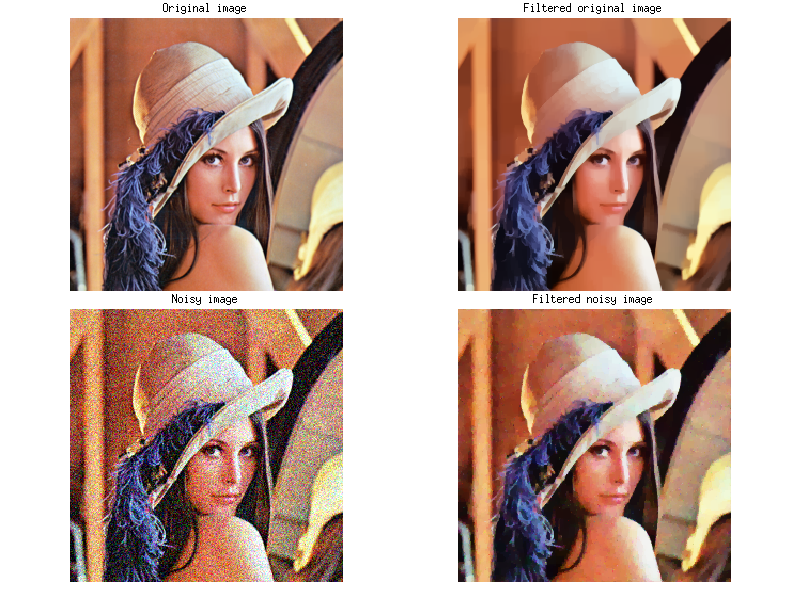
\includegraphics[width=0.6\textwidth]{images/TV_denoising.png}
    \caption{The result of Total Variation denoising}
    \label{fig:TVDenoising}
  \end{figure}
\end{frame}

\subsection {Richardson-Lucy}
\begin{frame}{Richardson-Lucy}
  The data model for the 1-D signal is:
  
  $$
  d_i = \sum\limits_{j}{p_{i, j}u_j},
  $$
  
  where $u_j$ is the intensity of the signal at the point $j$,
  $d_i$ is the detected intensity at the point $i$ and
  $p_{i, j}$ is a coefficient from the transition matrix P
  that describes the portion of signal from the source $j$
  that is detected in point $i$.
\end{frame}

\begin{frame}{Richardson-Lucy}
  In order to estimate $u_j$ if the PSF is known and we have 
  the observed signal $d_i$, we can begin iterative process
  that is described as follows:
  $$
  \hat{u}^{(t+1)}_j = \hat{u}^{(t)}_j\sum\limits_{i}
  \frac{d_i}{\sum\limits_{j}p_{ij}\hat{u}^{(t)}_j}p_{ij},
  $$
  where $t$ is the number of the iteration.
  
  We can rewrite the equation in terms of convolution with a PSF for the
  2-D signal the following way:
  $$
  \hat{u}^{(t+1)}=\hat{u}^{(t)}(\frac{d}{\hat{u}^{(t)} \otimes P} \otimes P^T),
  $$
  where $\otimes$ is a 2-D convolution of an image, $P^T$ is the 
  transposed PSF and the division and multiplication are element wise.
\end{frame}


\begin{frame}{Richardson-Lucy}
  We can introduce the Total Variation regularization to the process, if
  we rewrite the iterative equation as:
  
  $$
  \hat{u}^{(t+1)}=\frac{\hat{u}^{(t)}}{1 - \lambda V}
  (\frac{d}{\hat{u}^{(t)} \otimes P} \otimes P^T).
  $$
\end{frame}

\subsection {Wiener filtering}
\begin{frame}{Wiener}
  The data model for the signal is:
  
  $$
  y = hx + n,
  $$
  
  where $y$ is the resulting signal, $h$ is the Point Spread Function,
  $x$ is the unknown original signal and $n$ is the noise.
\end{frame}

\begin{frame}{Wiener}
  The Wiener filter in the frequency domain can be defined as
  $$
  G(f) = \frac{H^*(f)S(f)}{|H(f)|^2S(f)+N(f)},
  $$
  where:
  \begin{itemize}
    \item $G(f)$ and $H(f)$ are the Fourier transforms of 
      the Wiener deconvolution filter and the PSF,
    \item $S(f) = \mathop{\mathbb{E}|X(f)|^2}$ is the mean power spectral 
      density of the original signal $x$,
    \item $N(f) = \mathop{\mathbb{E}|X(f)|^2}$ is the mean power spectral 
      density of the noise $n$,
    \item $H^*(f)$ is the complex conjugation of $H(f)$.
  \end{itemize}
\end{frame}

\begin{frame}{Wiener}
  Thus, we can carry out the operation in the frequency domain as following:
  
  $$
  \hat{X(f)} = G(f)Y(f),
  $$
  and then perform an inverse Fourier transform, to obtain $x$.
\end{frame}

\section {Experiments}

\begin{frame}
  \tableofcontents[currentsection, subsectionstyle=show/show/hide]
\end{frame}

\subsection {Data}
\begin{frame}{Data}
  For the data, The Mouse hematopoietic stem cells in hydrogel microwells dataset from 
  the Cell Tracking Competition was used. The images are greyscale, 1010x1010 
  pixels in size.
  \begin{figure}
    \centering
    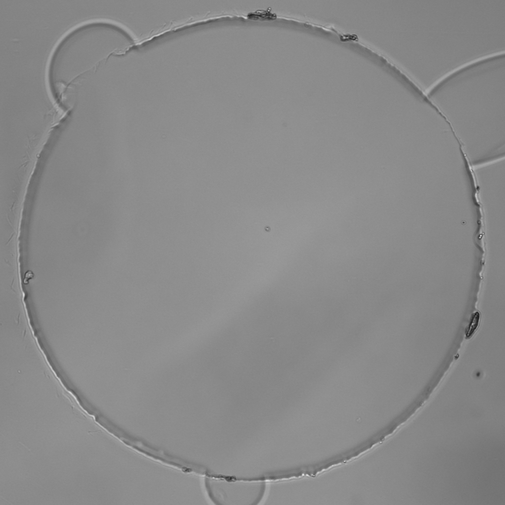
\includegraphics[width=0.35\textwidth]{images/cell.png}
    \caption{An example from the dataset, entropy is 4.8303}
    \label{fig:cell}
  \end{figure}
\end{frame}

\subsection{Preprocessing}
\begin{frame}{Preprocessing}
  Before exploring deconvolution methods, some preprocessing
  was done. According to the formulas, we have to apply some PSF
  to the images and then add some noise. 
  
  A gaussian blur kernel was used as the PSF function for the images. 
  Here is the result of blurring the image:
  \begin{figure}
    \centering
    
\includegraphics[width=0.30\textwidth]{images/blurred.png}
    \caption{Filter size is 5, sigma is 10, entropy is 19.4360}
    \label{fig:blurred}
  \end{figure}
\end{frame}

\begin{frame}{Preprocessing}
  
  \begin{figure}
    \centering
    \begin{subfigure}[t]{0.3\textwidth}
        
\includegraphics[width=\textwidth]{images/g_noise_low.png}
        \caption{Std = 0.01, \break entropy = 19.9601}
        \label{fig:noisy1}
    \end{subfigure}
    \begin{subfigure}[t]{0.3\textwidth}
        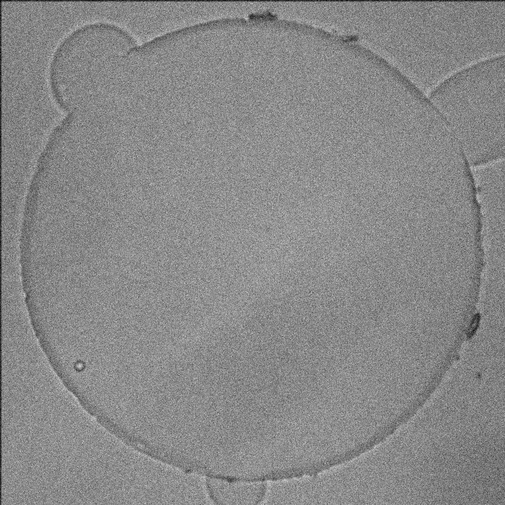
\includegraphics[width=\textwidth]{images/g_noise_mid.png}
        \caption{Std = 0.11, \break entropy = 19.9565}
        \label{fig:noisy2}
    \end{subfigure}
    \begin{subfigure}[t]{0.3\textwidth}
        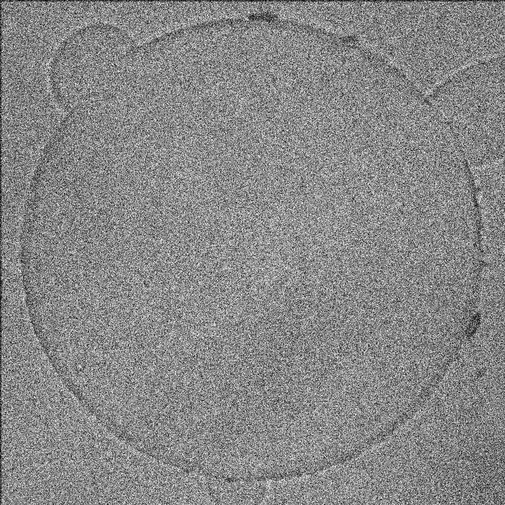
\includegraphics[width=\textwidth]{images/g_noise_high.png}
        \caption{Std = 0.3, \break entropy = 18.3776}
        \label{fig:noisy3}
    \end{subfigure}
    \caption{Images with different parameters of gaussian noise}
    \label{fig:images}
  \end{figure}
\end{frame}

\begin{frame}{Preprocessing}
  \begin{figure}
    \centering
    
\includegraphics[width=0.3\textwidth]{images/p_noise.png}
    \caption{An image with added poisson noise, entropy is 12.0254}
    \label{fig:poisson}
  \end{figure}
\end{frame}

\subsection{Restoration}
\begin{frame}{Restoration}
  
  \begin{figure}
    \centering
    \begin{subfigure}[t]{0.4\textwidth}
        
\includegraphics[width=0.8\textwidth]{images/unblurred_rl.png}
        \caption{Unblurred using Richardson-Lucy, \break SSIM = 0.9463, PSNR = 20.0621}
        \label{fig:restored}
    \end{subfigure}
    \begin{subfigure}[t]{0.4\textwidth}
        
\includegraphics[width=0.8\textwidth]{images/unblurred_w.png}
        \caption{Unblurred using Wiener, \break SSIM = 0.6798, PSNR = 18.0324}
        \label{fig:restored0}
    \end{subfigure}
    \caption{Deconvolutions of images without any noise}
  \end{figure}
\end{frame}

\begin{frame}{Restoration}
  \begin{figure}
    \centering
    \begin{subfigure}[t]{0.4\textwidth}
        
\includegraphics[width=0.8\textwidth]{images/unblurred_rl_low_noise.png}
        \caption{Unblurred using Richardson-Lucy, \break SSIM = 0.1808, PSNR = 16.7633}
        \label{fig:restored1}
    \end{subfigure}
    \begin{subfigure}[t]{0.4\textwidth}
        
\includegraphics[width=0.8\textwidth]{images/unblurred_w_low_noise.png}
        \caption{Unblurred using Wiener, \break SSIM = 0.7064, PSNR = 25.3072}
        \label{fig:restored2}
    \end{subfigure}
    \caption{Deconvolutions of images with gaussian noise with sigma = 0.01}
  \end{figure}
\end{frame}

\begin{frame}{Restoration}
  \begin{figure}
    \centering
    \begin{subfigure}[t]{0.4\textwidth}
        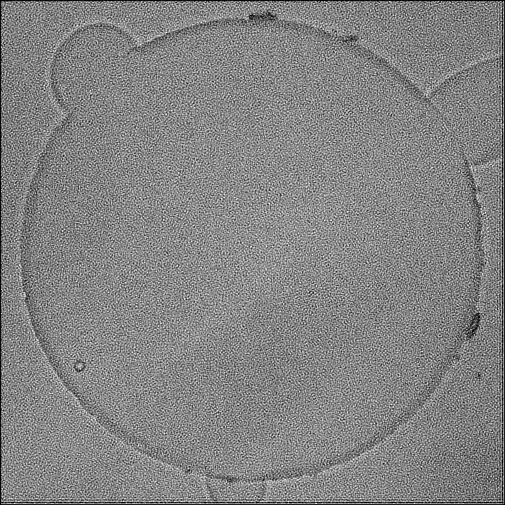
\includegraphics[width=0.8\textwidth]{images/unblurred_rl_mid_noise.png}
        \caption{Unblurred using Richardson-Lucy, \break SSIM = 0.0583, PSNR = 11.9206}
        \label{fig:restored5}
    \end{subfigure}
    \begin{subfigure}[t]{0.4\textwidth}
        
\includegraphics[width=0.8\textwidth]{images/unblurred_w_mid_noise.png}
        \caption{Unblurred using Wiener, \break SSIM = 0.5456, PSNR = 23.3830}
        \label{fig:restored6}
    \end{subfigure}
    \caption{Deconvolutions of images with gaussian noise with sigma = 0.11}
  \end{figure}
\end{frame}

\begin{frame}{Restoration}
  \begin{figure}
    \centering
    \begin{subfigure}[t]{0.4\textwidth}
        
\includegraphics[width=0.8\textwidth]{images/unblurred_rl_p_noise.png}
        \caption{Unblurred using Richardson-Lucy, \break SSIM = 0.0355, PSNR = 9.7349}
        \label{fig:restored9}
    \end{subfigure}
    \begin{subfigure}[t]{0.4\textwidth}
        
\includegraphics[width=0.8\textwidth]{images/unblurred_w_p_noise.png}
        \caption{Unblurred using Wiener, \break SSIM = 0.3611, PSNR = 13.4614}
        \label{fig:restored10}
    \end{subfigure}
    \caption{Deconvolutions of images with Poisson noise}
  \end{figure}
\end{frame}

\section{Conclusions}
\begin{frame}{Conclusions}
  \begin{itemize}
      \item Richardson-Lucy method of deconvolution has no
      edge effects on non-noisy images, opposed to Wiener filtering,
      \item Both PSNR and SSIM metrics are far better with Wiener filtering,
      \item Both Wiener filtering and Richardson-Lucy method
      are vulnerable to noise.
  \end{itemize}
  \begin{figure}
    \centering
    \begin{subfigure}[t]{0.4\textwidth}
        
\includegraphics[width=0.7\textwidth]{images/github_wiener.png}
        \caption{Github page with the code}
        \label{fig:restored9}
    \end{subfigure}
    \begin{subfigure}[t]{0.4\textwidth}
        
\includegraphics[width=0.7\textwidth]{images/notebook_wiener.png}
        \caption{HTML page for quick view of the notebook}
        \label{fig:restored10}
    \end{subfigure}
  \end{figure}
\end{frame}



\end{document}